\documentclass[10pt,journal,compsoc, onecolumn]{IEEEtran}
% 
% If IEEEtran.cls has not been installed into the LaTeX system files,
% manually specify the path to it like:
% \documentclass[10pt,journal,compsoc]{../sty/IEEEtran}

\usepackage{cite}
\usepackage[pdftex]{graphicx}
\DeclareGraphicsExtensions{.pdf,.jpeg,.png}
\usepackage{array}
\usepackage{amsmath}
\usepackage{amssymb}
\usepackage[table]{xcolor}       % 
\usepackage{colortbl}      %
\usepackage{mdwmath}
\usepackage{mdwtab}
\usepackage{eqparbox}
\usepackage{url}
\usepackage{hyperref}
\usepackage{multirow}
\usepackage{algorithm}
\usepackage{algpseudocode}
\usepackage{lineno} % 'switch' option for two-column documents
\usepackage{booktabs}
\usepackage{rotating} % Add this to your preamble

% Required Package
\usepackage[most]{tcolorbox}
\usepackage{enumitem}

% Define Colors
\definecolor{promptFrame}{HTML}{999999}
\definecolor{promptBody}{HTML}{f2f2f2}

% Table cell color shading (green=high, red=low accuracy)
\definecolor{cellHigh}{HTML}{2ca02c}    % green
\definecolor{cellMid}{HTML}{ffdd57}     % yellow
\definecolor{cellLow}{HTML}{d62728}     % red
% Accuracy shading: maps 40--100 to red-yellow-green (using pgfmath for robust expansion in tabular)
\newcommand{\acc}[1]{%
  \pgfmathtruncatemacro{\acclevel}{#1 < 60 ? 1 : (#1 < 75 ? 2 : (#1 < 85 ? 3 : 4))}%
  \ifnum\acclevel=1 \cellcolor{cellLow!40}\fi
  \ifnum\acclevel=2 \cellcolor{cellMid!40}\fi
  \ifnum\acclevel=3 \cellcolor{cellMid!20}\fi
  \ifnum\acclevel=4 \cellcolor{cellHigh!25}\fi
  #1}
% Best-in-row bold wrapper
\newcommand{\best}[1]{\textbf{#1}}

% brief communications 
% Abstract – up to 150 words, unreferenced. 
% Main text – up to 2,000 words, including abstract, references and figure legends, and contains no headings. 
% Display items – up to 2 items, although this may be flexible at the discretion of the editor, provided the page limit is observed. 
% Online Methods section should be included.
% References - as a guideline, we typically recommend up to 20. Article titles are omitted from the reference list.

% correct bad hyphenation here
\hyphenation{op-tical net-works semi-conduc-tor}

% Brief Communication in Nature Medicine https://www.nature.com/nm/content

\begin{document}

% \linenumbers
\title{Benchmarking and Adapting On-Device Large Language Models for Clinical Decision Support}
%


\author{Alif Munim$^*$, Omar Ibrahim$^*$, Alhusain Abdalla$^*$, Jun Ma$^*$, Meng Wei, Shuolin Yin, Leo Chen, and Bo Wang % <-this % stops a space


\IEEEcompsocitemizethanks{
\IEEEcompsocthanksitem Alif Munim is with AI Collaborative Centre, University Health Network, Toronto, Canada. ($*$ Equal Contribution)
% \protect\\
% note need leading \protect in front of \\ to get a newline within \thanks as
% \\ is fragile and will error, could use \hfil\break instead.
\IEEEcompsocthanksitem Omar Ibrahim is with AI Collaborative Centre, University Health Network, Toronto, Canada. ($*$ Equal Contribution)
\IEEEcompsocthanksitem Alhusain Abdalla is with AI Collaborative Centre, University Health Network, Toronto, Canada. ($*$ Equal Contribution)
\IEEEcompsocthanksitem Jun Ma is with AI Collaborative Centre and Princess Margaret Cancer Centre, University Health Network, Toronto, Canada. ($*$ Equal Contribution)
\IEEEcompsocthanksitem Shuolin Yin is with Department of Electrical and Computer Engineering, University of Toronto, Toronto, Canada.
\IEEEcompsocthanksitem Leo Chen is with Division of Urology, Department of Surgery, St. Michael’s Hospital, Unity Health Toronto and University of Toronto, Toronto, Canada
\IEEEcompsocthanksitem Bo Wang (Corresponding Author) is with Peter Munk Cardiac Centre, University Health Network; Department of Laboratory Medicine and Pathobiology and Department of Computer Science, University of Toronto;  Vector Institute, Toronto, Canada. 
E-mail: bowang@vectorinstitute.ai}% <-this % stops an unwanted space
}

\IEEEtitleabstractindextext{%
\begin{abstract}
Large language models (LLMs) have rapidly advanced in clinical decision-making, yet the deployment of proprietary systems is hindered by privacy concerns and reliance on cloud-based infrastructure. Open-source alternatives allow local inference but often have large model sizes that limit their use in resource-constrained clinical settings. Here, we benchmark on-device LLMs from the gpt-oss (20b, 120b), Qwen3.5 (9B, 27B, 35B), and Gemma 4 (31B) families across three representative clinical tasks: general disease diagnosis, specialty-specific (ophthalmology) diagnosis and management, and simulation of human expert grading and evaluation. We compare their performance with state-of-the-art proprietary models (GPT-5.1, GPT-5-mini, and Gemini 3.1 Pro) and a leading open-source model (DeepSeek-R1), and we further evaluate the adaptability of on-device systems by fine-tuning gpt-oss-20b and Qwen3.5-35B on general diagnostic data. Across tasks, on-device models achieve performance comparable to or exceeding DeepSeek-R1 and GPT-5-mini despite being substantially smaller. In addition, fine-tuning remarkably improves diagnostic accuracy, with the fine-tuned Qwen3.5-35B reaching 88.4\% and approaching the proprietary GPT-5.1 (88.9\%). Among base on-device models, Gemma 4 31B achieved the strongest general diagnostic accuracy at 86.5\%, exceeding GPT-5-mini and approaching the fine-tuned Qwen3.5-35B. These findings highlight the potential of on-device LLMs to deliver accurate, adaptable, and privacy-preserving clinical decision support, offering a practical pathway for broader integration of LLMs into routine clinical practice.
\end{abstract}

%%
}

\maketitle



\IEEEdisplaynontitleabstractindextext
% \IEEEdisplaynontitleabstractindextext has no effect when using
% compsoc or transmag under a non-conference mode.

% up to 2000 words 

% For peer review papers, this IEEEtran command inserts a page break and
% creates the second title. It will be ignored for other modes.
\IEEEpeerreviewmaketitle

\section*{Introduction}
% general background
Large language models (LLMs) are rapidly transforming the landscape of clinical medicine~\cite{thirunavukarasu2023llmedicine, omiye2024pitfalls}. Trained on massive corpora of general-domain and biomedical text, these models have demonstrated emergent reasoning abilities that enable comprehensive summaries from medical dialogue~\cite{NMed-LLMSummary}, disease diagnosis, and treatment planning~\cite{MedFound}. For example, Med-PaLM~\cite{MedPALM1,MedPALM2} and AMIE~\cite{AMIE-diagnosis,AMIE-conversation} achieved near-clinician performance in open-ended medical question answering, differential diagnosis, and patient consultation simulations~\cite{qiu2025medrench}. In real-world evaluations~\cite{openai-AIConsult, goh2025gpt4rct}, LLM-assisted physicians exhibited improved diagnostic accuracy and management decisions across diverse clinical scenarios. Together, these advances illustrate the growing potential of LLMs to augment clinical expertise and support decision-making at the point of care.

% limitation of proprietary LLMs
Despite these achievements, the translation of LLMs into real-world clinical workflows remains limited~\cite{hager2024limitations}. Most frontier LLMs are proprietary, cloud-hosted, and trained on non-transparent datasets, creating challenges related to data privacy, regulatory compliance, reproducibility, and cost. The transmission of patient information to external servers conflicts with data-governance policies in many health institutions~\cite{kim2025privacy, clusmann2025implementing}. Moreover, the high cost associated with developing, training, and deploying large-scale proprietary models can be prohibitive for many healthcare institutions. 

% limitation of public LLMs
The open-source community has developed increasingly capable models that approach the performance of proprietary systems while allowing full local control. Models such as DeepSeek-R1~\cite{DeepSeek-R1} have demonstrated competitive reasoning and clinical comprehension across diagnostic and treatment-related tasks~\cite{eval-deepseek,eval-deepseek125Patients, wang2025jarvis, moell2025deepseek, deepseek2025cme}. 
However, the adoption of DeepSeek-R1 in clinical environments is constrained because of the large model size of 671 billion parameters, which requires substantial computational costs. The models of this scale not only hinder deployment in clinics with limited access to computing resources, but also make fine-tuning for adaptation in evolving clinical domains prohibitively expensive. 
These limitations underscore the need for smaller, efficient models that retain clinical reasoning ability while remaining feasible for on-premise use~\cite{garg2025rise, builtjes2025leveraging}.


% our contributions 
The recent advancements in on-device LLMs offer a promising solution to the challenges posed by both large proprietary and open-source models~\cite{zhu2025empowering, evangelista2026graphrag}. In particular, the gpt-oss family~\cite{gpt-oss} represents this new generation of efficient and privacy-preserving architectures. The gpt-oss-20b model and its larger counterpart, gpt-oss-120b, are designed and optimized for deployment on a single consumer GPU with 16GB and 80GB memory, respectively. Similarly, the Qwen3.5 family of open-weight models (9B, 27B, and 35B parameters) offers an alternative on-device architecture suitable for resource-constrained deployment.
This study aims to determine whether on-device LLMs can be practically used for clinical decision support. We systematically benchmark gpt-oss (20b, 120b) and Qwen3.5 (9B, 27B, 35B) models across three representative tasks: general disease diagnosis, (ophthalmology) specialty-specific disease diagnosis and management, and simulation of human clinician judgement and evaluation (Fig.~\ref{fig:1}). To establish a clear performance landscape, we compare these on-device models against leading proprietary models (GPT-5.1, GPT-5-mini, and Gemini 3.1 Pro) and a strong open-source model (DeepSeek-R1). 


\begin{figure}[htbp]
\centering
% Changed scale to width to ensure it stays within the text margins
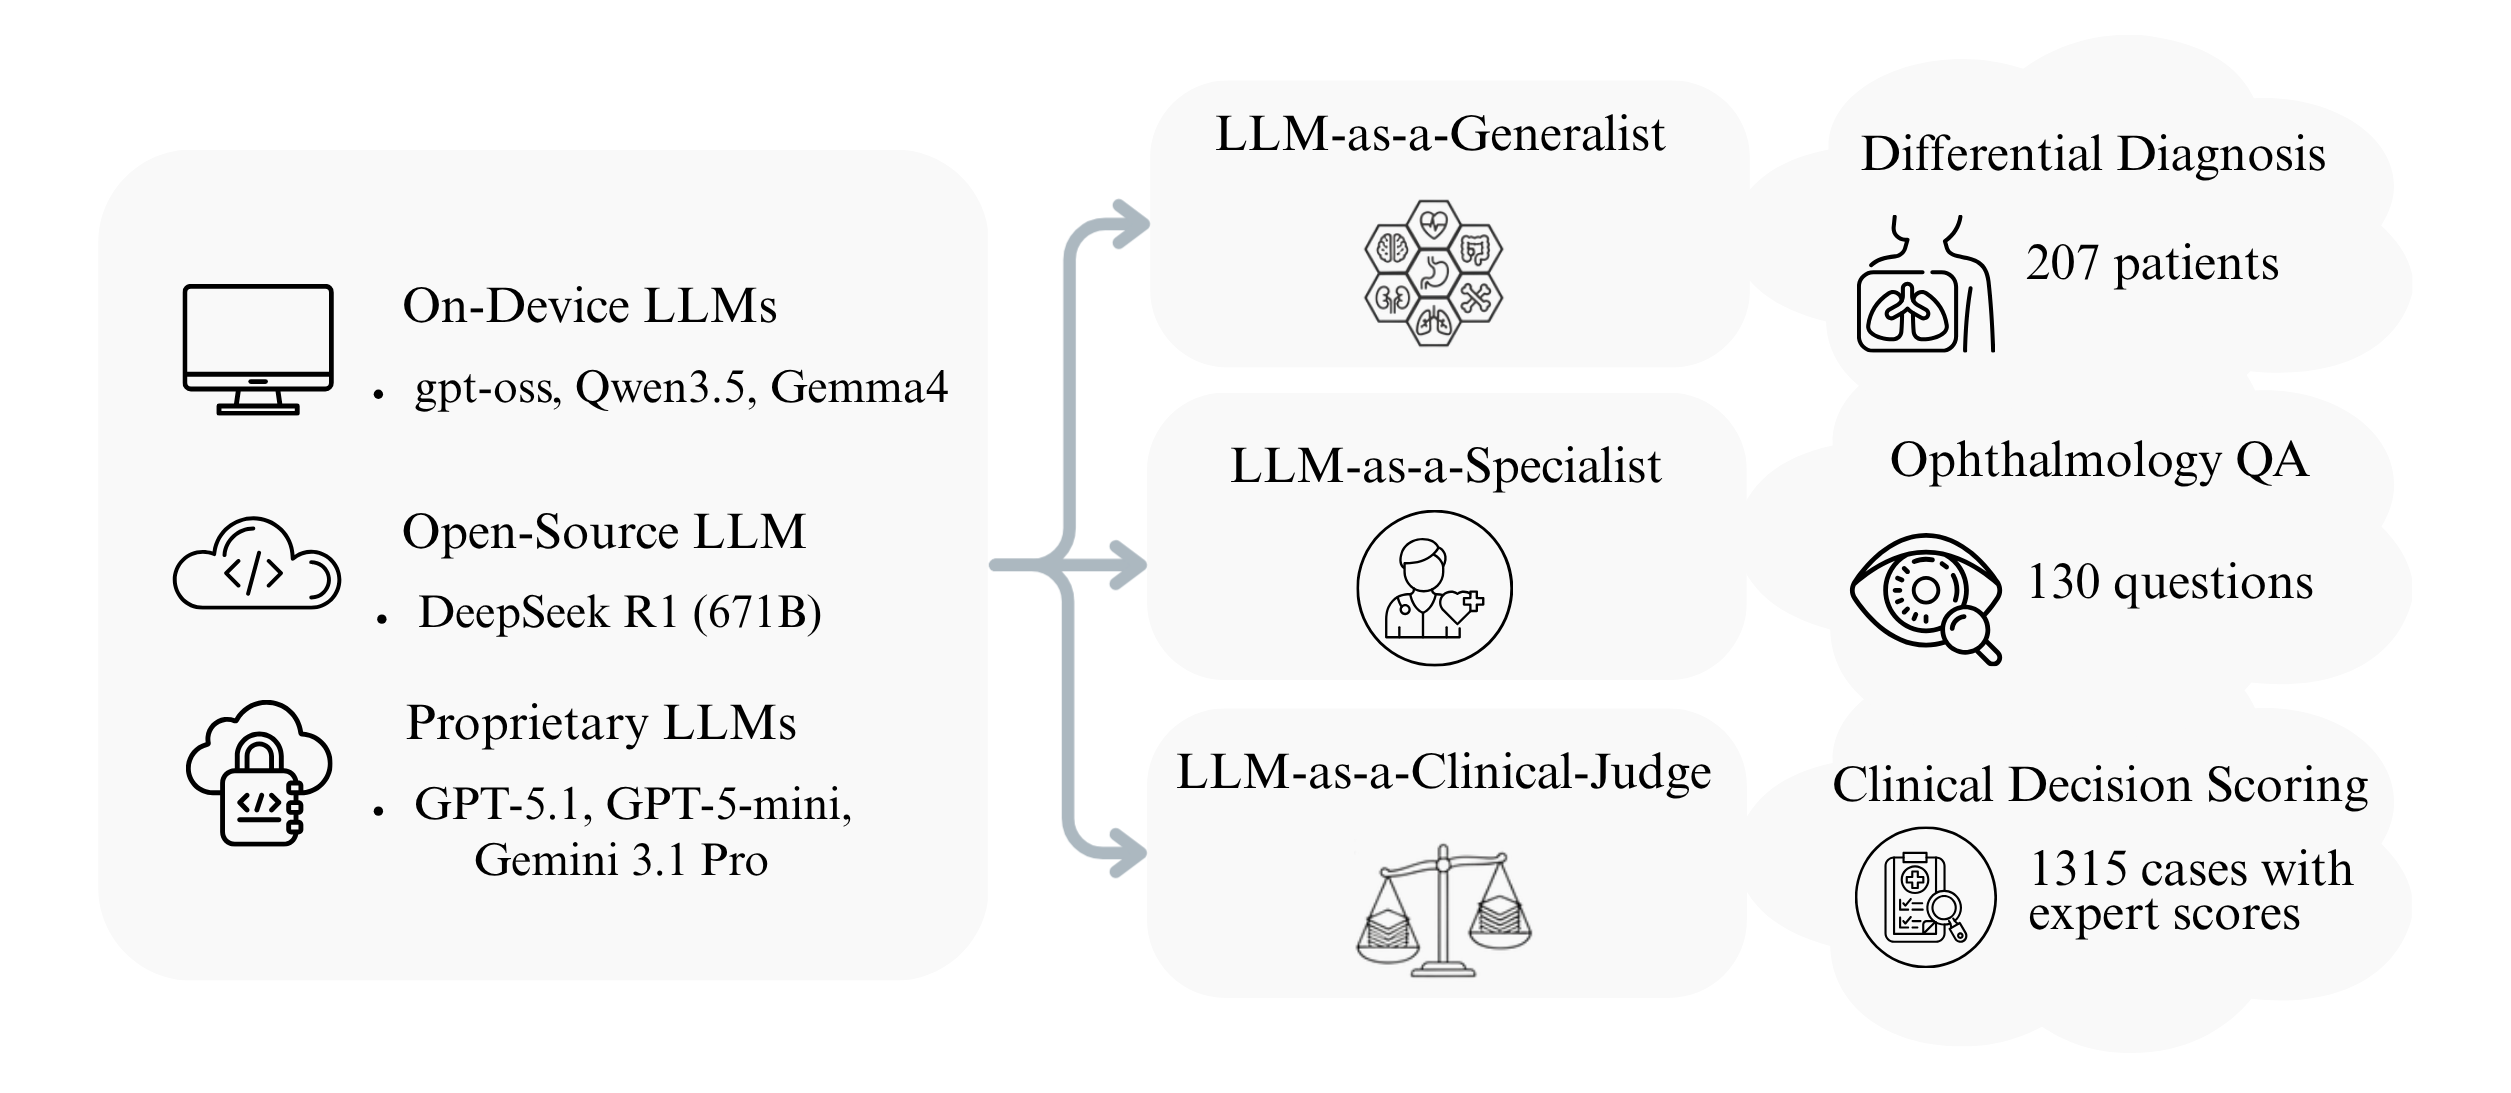
\includegraphics[width=\textwidth]{main-imgs/fig1.png} 
\caption{\textbf{Overview of the benchmark framework.} This study compares on-device LLMs (gpt-oss and Qwen3.5) with state-of-the-art open-source (DeepSeek-R1) and proprietary LLMs (GPT-5.1, GPT-5-mini, Gemini 3.1 Pro) across general disease diagnosis, specialty diagnosis and management (ophthalmology), and clinical judgment simulation.}
\label{fig:1}
\end{figure}



\section*{Results}
% data set introduction
\subsection*{Dataset and evaluation methods} 
We mainly focus on assessing the performance of LLMs on disease diagnosis, treatment recommendations, and simulating expert judgment for open-ended questions, as these are common tasks in clinical practice. We curated three datasets and benchmarked model performance on three scenarios: LLM-as-a-generalist, LLM-as-a-specialist, and LLM-as-a-clinical-judge (Fig.~\ref{fig:1}).  

Specifically, to assess the capability of LLMs for general disease diagnosis, we collected 207 case reports from the Eurorad library~\cite{kottlors2025eurorad} where each case contains clinical history, findings from associated medical images (e.g., computed tomography (CT), magnetic resonance imaging  (MRI), and ultrasound), and a fine-grained differential diagnosis list (Methods). The task is to select the diagnosis from the list based on patient history and imaging findings (Supplementary Prompt 1). 

The second dataset was from an ophthalmology multiple-choice question dataset~\cite{ophthalmologyQA}, aiming to evaluate the specialty-specific performance of LLMs (Methods). The dataset contains 39 diagnosis questions and 91 management questions. Each question contains patient sex, age, and examinations findings, such as visual acuity, intraocular pressure, and fundus examinations, and a list of five to nine answer options. The task is to select correct answers, and each question may have multiple correct answers (Supplementary Prompt 2).  

The third dataset was adapted from the existing benchmarking study of the DeepSeek-R1 model~\cite{eval-deepseek125Patients}, including 1315 cases with human expert scores from 125 patients across five specialties (internal medicine, neurology, surgery, gynecology, and pediatrics) (Methods). LLMs are tasked to simulate human experts to assess given diagnoses from existing LLMs and assign a score from 1 to 5 based on a predefined rubric. We compare these LLM-generated scores against ground-truth human expert scores  (Supplementary Prompt 3-4). 

 For the LLM-as-a-generalist and LLM-as-a-specialist tasks, the evaluation was based on exact match accuracy. For the LLM-as-a-clinical-judge task, we computed the relative error between the clinicians' scores and the LLM's scores. 
To ensure rigorous zero-shot evaluation and prevent data leakage, all three benchmark datasets were curated from cases released after the training data cutoff for all evaluated LLMs. 


\begin{figure}[!htbp]
\centering
\enlargethispage{2cm}
\vspace*{-1.5cm}
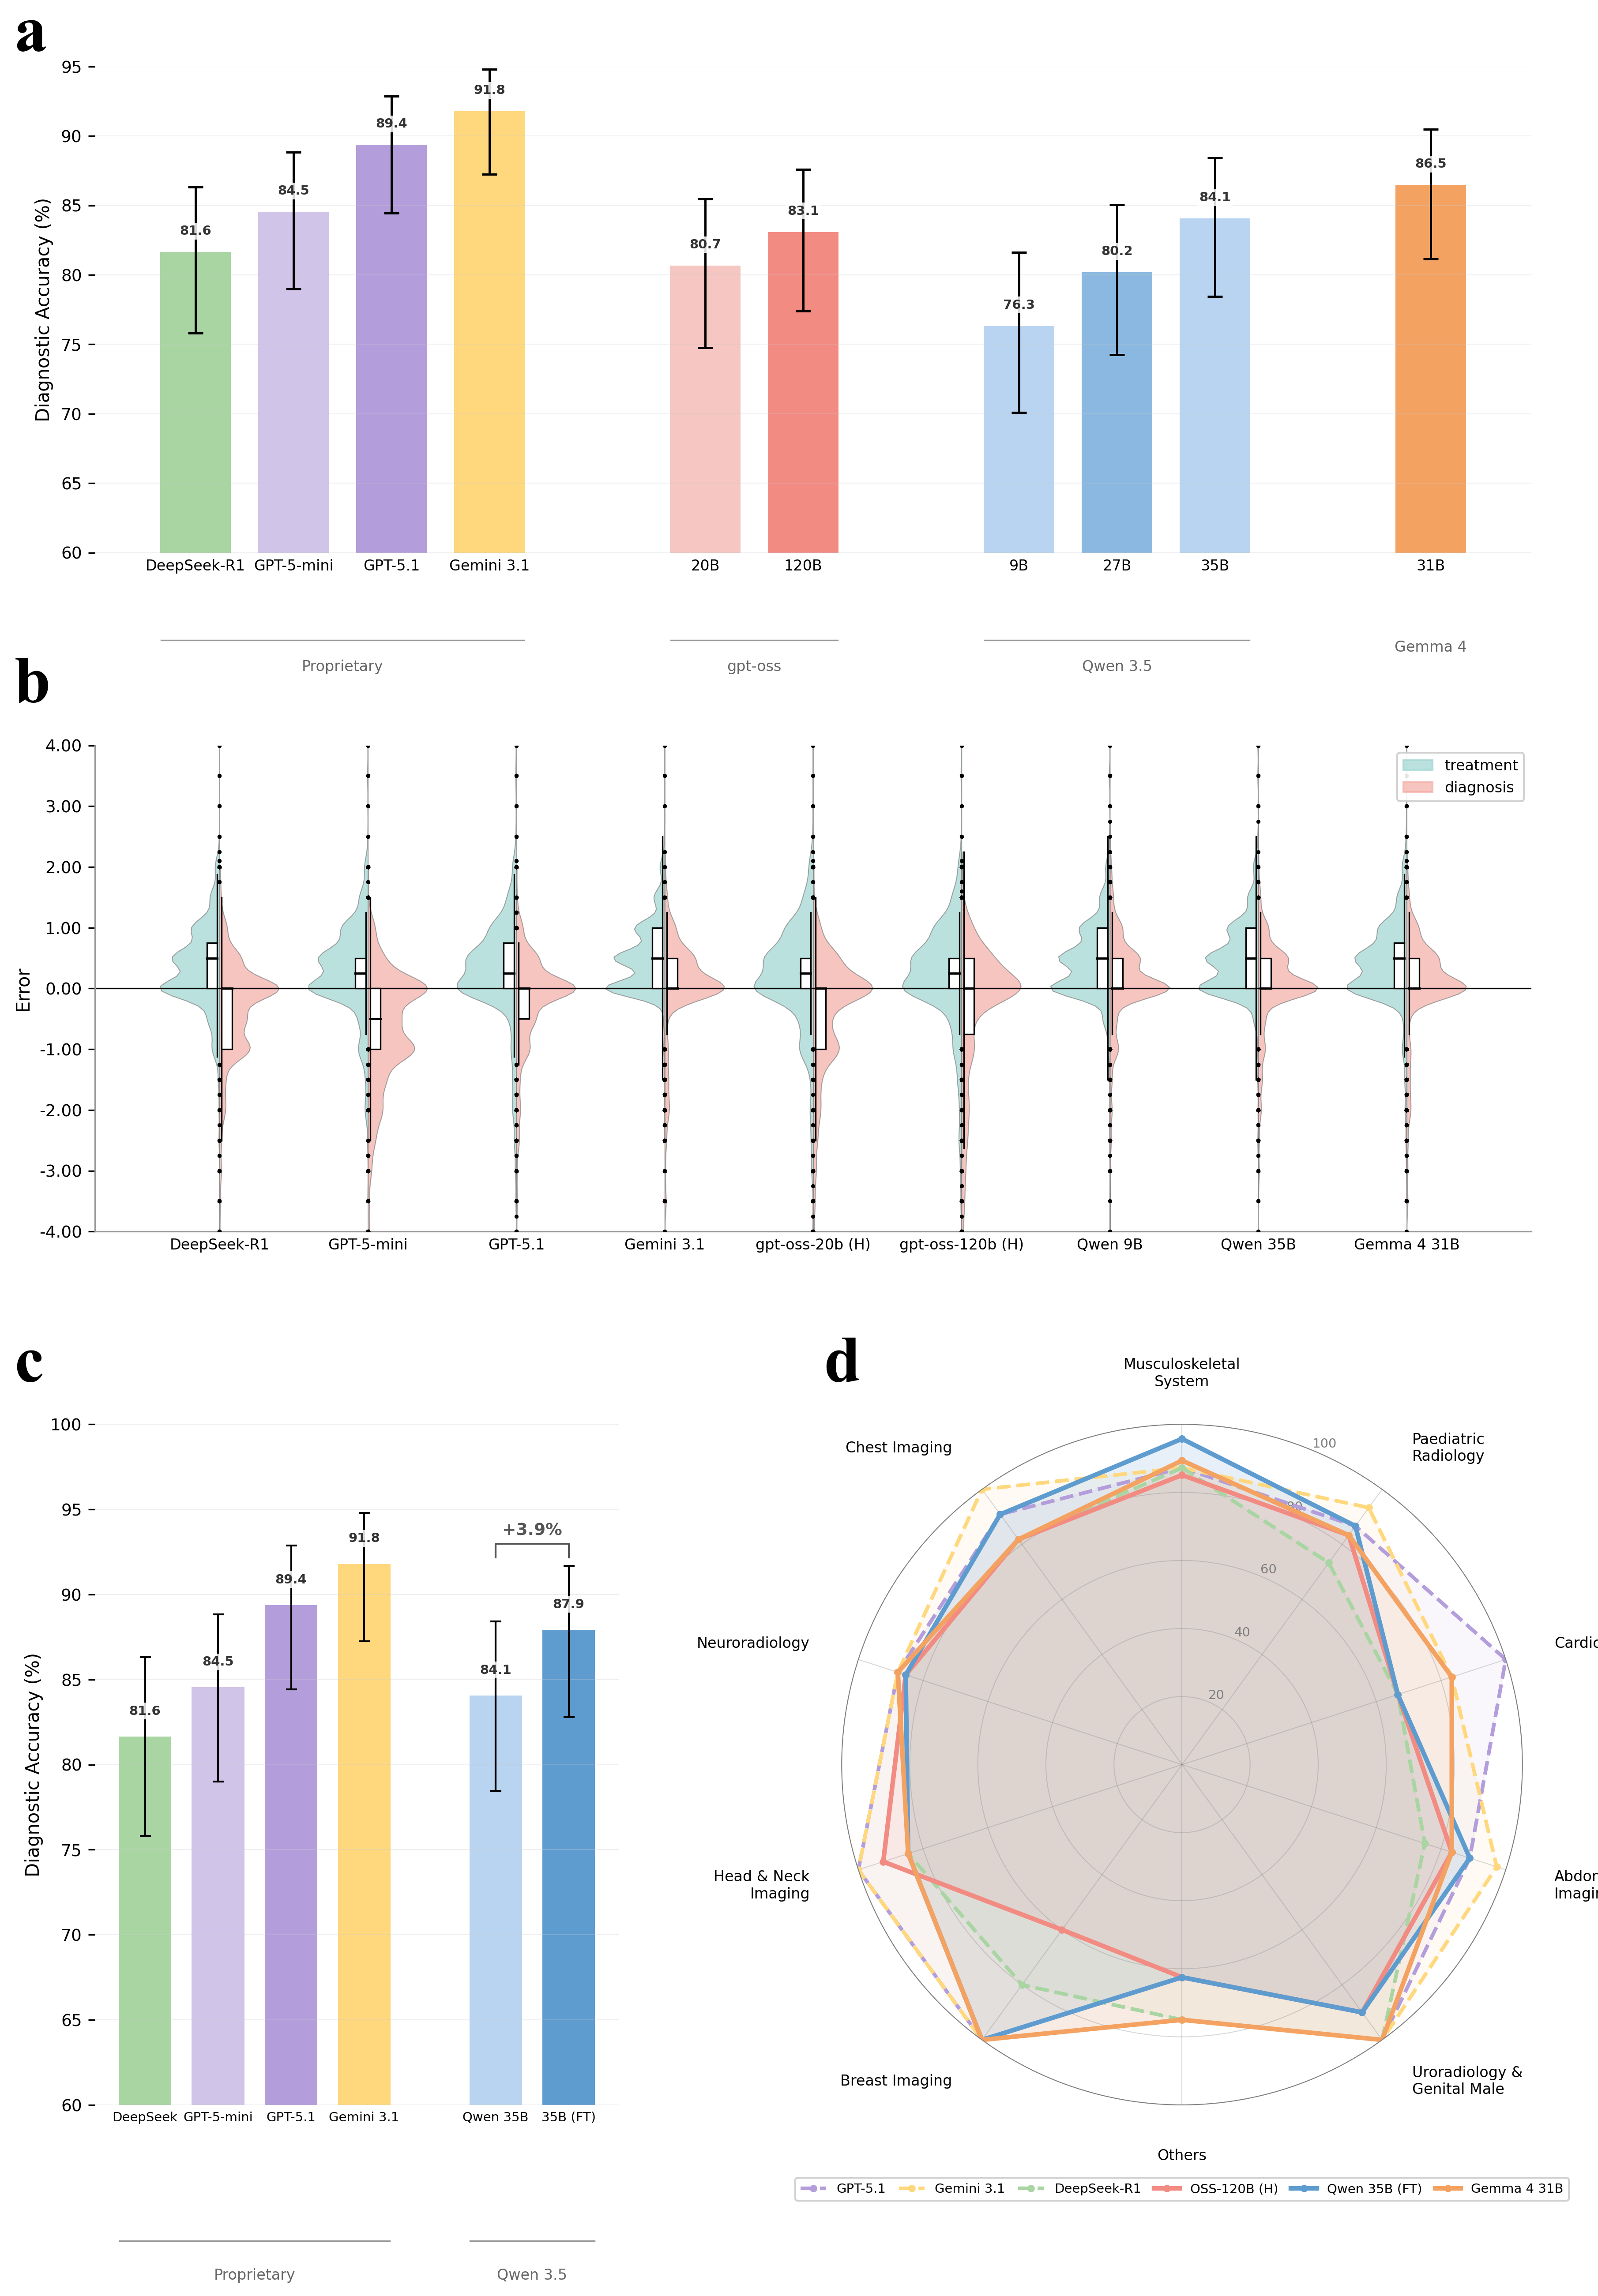
\includegraphics[width=\textwidth,height=0.92\textheight,keepaspectratio]{main-imgs/fig2_combined.png}
\caption{\textbf{Zero-shot and fine-tuning performance of on-device LLMs.}
\textbf{a,} Results of LLM-as-a-generalist: diagnosis accuracy on a wide range of radiological cases (N=207).
\textbf{b,} Results of LLM-as-a-clinical-judge: violin plots comparing the relative error for disease diagnosis and treatment open-ended question assessment (N=1315).
\textbf{c,} Fine-tuned Qwen3.5-35B model accuracy compared to proprietary LLMs on the disease differential diagnosis task.
\textbf{d,} Model performance across 10 radiological sub-specialties.
}\label{fig:2}
\end{figure}

\begin{table}[!htbp]
\centering
\scriptsize
\setlength{\tabcolsep}{3pt}
\caption{\textbf{LLM-as-a-Generalist Task: Comparative diagnostic accuracy (\%) across radiological anatomical subgroups.}
Performance is evaluated using self-consistency majority voting. The best result per row is \textbf{bolded}. Full 95\% CIs are provided in Supplementary Table~1.}
\label{tab:generalist_results}
\begin{tabular}{l ccc @{\hskip 6pt} c @{\hskip 6pt} cc @{\hskip 6pt} cccc @{\hskip 6pt} c}
\toprule
& \multicolumn{3}{c}{\textbf{Proprietary}} & \textbf{Open} & \multicolumn{2}{c}{\textbf{gpt-oss}} & \multicolumn{4}{c}{\textbf{Qwen3.5}} & \textbf{Gemma 4} \\
\cmidrule(lr){2-4} \cmidrule(lr){5-5} \cmidrule(lr){6-7} \cmidrule(lr){8-11} \cmidrule(lr){12-12}
\textbf{Category} &
\textbf{GPT-5.1} & \textbf{GPT-5-mini} & \textbf{Gemini-3.1} & \textbf{DS-R1} &
\textbf{20b} & \textbf{120b} &
\textbf{9B} & \textbf{27B} & \textbf{35B} & \textbf{35B-FT} & \textbf{31B} \\
\midrule
Musculoskeletal   & \acc{87.2} & \acc{83.0} & \acc{87.2} & \acc{87.2} & \acc{87.2} & \acc{85.1} & \acc{89.4} & \acc{87.2} & \acc{89.4} & \best{\acc{95.7}} & \acc{89.4} \\
Cardiovascular    & \best{\acc{83.3}} & \acc{66.7} & \acc{66.7} & \acc{66.7} & \acc{50.0} & \acc{66.7} & \acc{50.0} & \acc{50.0} & \acc{66.7} & \best{\acc{83.3}} & \best{\acc{83.3}} \\
Abdominal         & \acc{88.9} & \acc{88.9} & \best{\acc{97.2}} & \acc{75.0} & \acc{80.6} & \acc{83.3} & \acc{72.2} & \acc{83.3} & \acc{83.3} & \acc{88.9} & \acc{83.3} \\
Uroradiology      & \best{\acc{100.0}} & \acc{90.0} & \best{\acc{100.0}} & \best{\acc{100.0}} & \best{\acc{100.0}} & \acc{90.0} & \best{\acc{100.0}} & \acc{90.0} & \best{\acc{100.0}} & \acc{90.0} & \best{\acc{100.0}} \\
Neuroradiology    & \best{\acc{87.8}} & \acc{82.9} & \best{\acc{87.8}} & \acc{85.4} & \acc{85.4} & \acc{85.4} & \acc{70.7} & \acc{78.0} & \acc{82.9} & \acc{85.4} & \best{\acc{87.8}} \\
Paediatric        & \acc{86.7} & \acc{80.0} & \best{\acc{93.3}} & \acc{73.3} & \acc{70.0} & \acc{83.3} & \acc{63.3} & \acc{70.0} & \acc{80.0} & \acc{86.7} & \acc{83.3} \\
Head \& neck      & \best{\acc{100.0}} & \best{\acc{100.0}} & \best{\acc{100.0}} & \acc{84.6} & \acc{92.3} & \acc{92.3} & \acc{84.6} & \acc{92.3} & \acc{92.3} & \acc{84.6} & \acc{84.6} \\
Breast            & \best{\acc{100.0}} & \acc{80.0} & \best{\acc{100.0}} & \acc{80.0} & \acc{40.0} & \acc{60.0} & \acc{80.0} & \best{\acc{100.0}} & \best{\acc{100.0}} & \best{\acc{100.0}} & \best{\acc{100.0}} \\
Chest             & \acc{90.9} & \acc{81.8} & \best{\acc{100.0}} & \acc{81.8} & \acc{81.8} & \acc{81.8} & \acc{63.6} & \acc{63.6} & \acc{72.7} & \acc{90.9} & \acc{81.8} \\
Others            & \best{\acc{75.0}} & \best{\acc{75.0}} & \best{\acc{75.0}} & \best{\acc{75.0}} & \acc{62.5} & \acc{62.5} & \best{\acc{75.0}} & \best{\acc{75.0}} & \best{\acc{75.0}} & \acc{62.5} & \best{\acc{75.0}} \\
\midrule
\textbf{Average}  & \acc{88.9} & \acc{84.1} & \best{\acc{91.3}} & \acc{81.6} & \acc{80.7} & \acc{83.1} & \acc{75.8} & \acc{80.2} & \acc{84.5} & \acc{88.4} & \acc{86.5} \\
\bottomrule
\end{tabular}
\end{table}


\subsection*{On-device LLMs show competitive zero-shot performance}
Fig.~\ref{fig:2}a and Table~\ref{tab:generalist_results} compare the diagnostic accuracy of the evaluated models for general disease diagnosis across radiological case reports. Among the proprietary frontier models, Gemini 3.1 Pro achieved the highest overall accuracy of 91.3\% (95\% CI: 86.7--94.4\%), followed by GPT-5.1 at 88.9\% (95\% CI: 83.9--92.5\%). The on-device models demonstrated strong competitiveness relative to these baselines. Specifically, the gpt-oss-120b (H) model achieved an accuracy of 83.1\% (95\% CI: 77.4--87.6\%), while the highly efficient gpt-oss-20b (H) model secured 80.7\% (95\% CI: 74.8--85.5\%), matching the performance of the significantly larger DeepSeek-R1 (81.6\%; 95\% CI: 75.8--86.3\%; $p>0.05$). Among the Qwen3.5 on-device models, the 35B variant achieved the highest base accuracy at 84.5\% (95\% CI: 79.0--88.8\%), matching GPT-5-mini (84.1\%; 95\% CI: 78.5--88.4\%; $p>0.05$) and exceeding DeepSeek-R1. The Qwen3.5 27B model achieved 80.2\% (95\% CI: 74.2--85.1\%), comparable to both gpt-oss-20b (H) and DeepSeek-R1 ($p>0.05$), while the smallest 9B variant reached 75.8\% (95\% CI: 69.6--81.2\%).

Gemma 4 31B achieved the strongest base on-device accuracy at 86.5\% (95\% CI: 81.1--90.5\%), exceeding GPT-5-mini (84.1\%; $p>0.05$) and surpassing the strongest Qwen3.5 base variant (35B, 84.5\%) by 2.0 percentage points. This result places Gemma 4 31B between GPT-5-mini and GPT-5.1 (88.9\%) on the general diagnosis task, and significantly above Qwen3.5 9B ($p<0.05$). Subspecialty analysis (Table~\ref{tab:generalist_results}) shows uniformly strong performance, with perfect scores on uroradiology and breast imaging.



\begin{table}[!htbp]
\centering
\scriptsize
\setlength{\tabcolsep}{3.5pt}
\caption{\textbf{LLM-as-a-Specialist Task: Comparative accuracy (\%) on ophthalmology diagnosis and management tasks.} The best result per row is \textbf{bolded}. Full 95\% CIs are provided in Supplementary Table~2.}
\label{tab:ophthalmology_results}
\begin{tabular}{ll ccc @{\hskip 6pt} c @{\hskip 6pt} ccc @{\hskip 6pt} ccc @{\hskip 6pt} ccc @{\hskip 6pt} c}
\toprule
& & \multicolumn{3}{c}{\textbf{Proprietary}} & \textbf{Open} & \multicolumn{3}{c}{\textbf{gpt-oss-20b}} & \multicolumn{3}{c}{\textbf{gpt-oss-120b}} & \multicolumn{3}{c}{\textbf{Qwen3.5}} & \textbf{Gemma 4} \\
\cmidrule(lr){3-5} \cmidrule(lr){6-6} \cmidrule(lr){7-9} \cmidrule(lr){10-12} \cmidrule(lr){13-15} \cmidrule(lr){16-16}
\textbf{Type} & \textbf{Topic} & \textbf{GPT-5.1} & \textbf{GPT-5-mini} & \textbf{Gemini-3.1} & \textbf{DS-R1} & \textbf{L} & \textbf{M} & \textbf{H} & \textbf{L} & \textbf{M} & \textbf{H} & \textbf{35B} & \textbf{27B} & \textbf{9B} & \textbf{31B} \\
\midrule
\multirow{6}{*}{\rotatebox{90}{\textbf{Diagnosis}}}
& Glaucoma           & \best{\acc{100.0}} & \best{\acc{100.0}} & \best{\acc{100.0}} & \best{\acc{100.0}} & \acc{71.4} & \acc{85.7} & \acc{85.7} & \acc{85.7} & \acc{85.7} & \acc{85.7} & \best{\acc{100.0}} & \best{\acc{100.0}} & \best{\acc{100.0}} & \acc{85.7} \\
& Ext.\ Eye/Orbital  & \best{\acc{90.0}} & \acc{80.0} & \best{\acc{90.0}} & \best{\acc{90.0}} & \acc{70.0} & \acc{70.0} & \acc{80.0} & \acc{70.0} & \acc{80.0} & \acc{80.0} & \acc{70.0} & \acc{70.0} & \acc{70.0} & \acc{80.0} \\
& Retinal            & \best{\acc{100.0}} & \best{\acc{100.0}} & \best{\acc{100.0}} & \best{\acc{100.0}} & \acc{66.7} & \acc{66.7} & \acc{66.7} & \best{\acc{100.0}} & \acc{66.7} & \acc{66.7} & \best{\acc{100.0}} & \best{\acc{100.0}} & \acc{66.7} & \acc{66.7} \\
& Anterior Segment   & \acc{50.0} & \best{\acc{75.0}} & \best{\acc{75.0}} & \best{\acc{75.0}} & \acc{62.5} & \acc{62.5} & \acc{62.5} & \best{\acc{75.0}} & \best{\acc{75.0}} & \best{\acc{75.0}} & \best{\acc{75.0}} & \best{\acc{87.5}} & \best{\acc{75.0}} & \best{\acc{75.0}} \\
& Ocular Trauma      & \best{\acc{100.0}} & \acc{83.3} & \best{\acc{100.0}} & \best{\acc{100.0}} & \acc{83.3} & \acc{66.7} & \acc{83.3} & \acc{83.3} & \best{\acc{100.0}} & \acc{83.3} & \best{\acc{100.0}} & \best{\acc{100.0}} & \acc{83.3} & \best{\acc{100.0}} \\
& Refract./Strabismus & \best{\acc{100.0}} & \best{\acc{100.0}} & \best{\acc{100.0}} & \best{\acc{100.0}} & \best{\acc{100.0}} & \best{\acc{100.0}} & \best{\acc{100.0}} & \best{\acc{100.0}} & \best{\acc{100.0}} & \best{\acc{100.0}} & \best{\acc{100.0}} & \best{\acc{100.0}} & \best{\acc{100.0}} & \best{\acc{100.0}} \\
\cmidrule{2-16}
& \textit{Average}   & \textit{\acc{87.2}} & \textit{\acc{87.2}} & \textit{\best{\acc{92.3}}} & \textit{\best{\acc{92.3}}} & \textit{\acc{74.4}} & \textit{\acc{74.4}} & \textit{\acc{79.5}} & \textit{\acc{82.1}} & \textit{\acc{84.6}} & \textit{\acc{82.1}} & \textit{\acc{87.2}} & \textit{\best{\acc{89.7}}} & \textit{\acc{82.1}} & \textit{\acc{84.6}} \\
\midrule
\multirow{6}{*}{\rotatebox{90}{\textbf{Mgmt}}}
& Glaucoma           & \best{\acc{85.7}} & \acc{64.3} & \best{\acc{85.7}} & \acc{71.4} & \acc{50.0} & \acc{64.3} & \acc{50.0} & \acc{71.4} & \acc{78.6} & \acc{64.3} & \best{\acc{85.7}} & \best{\acc{85.7}} & \acc{64.3} & \acc{71.4} \\
& Ext.\ Eye/Orbital  & \acc{71.4} & \acc{57.1} & \acc{64.3} & \acc{78.6} & \acc{57.1} & \acc{71.4} & \acc{64.3} & \acc{71.4} & \acc{71.4} & \acc{71.4} & \best{\acc{92.9}} & \acc{71.4} & \acc{78.6} & \acc{78.6} \\
& Retinal            & \acc{37.5} & \acc{25.0} & \acc{37.5} & \acc{37.5} & \acc{12.5} & \acc{25.0} & \acc{37.5} & \best{\acc{50.0}} & \acc{37.5} & \acc{37.5} & \acc{37.5} & \acc{25.0} & \acc{37.5} & \acc{37.5} \\
& Anterior Segment   & \best{\acc{82.4}} & \acc{64.7} & \best{\acc{82.4}} & \acc{70.6} & \acc{76.5} & \acc{64.7} & \acc{76.5} & \acc{70.6} & \acc{76.5} & \acc{70.6} & \acc{64.7} & \acc{64.7} & \acc{58.8} & \acc{58.8} \\
& Ocular Trauma      & \acc{65.4} & \acc{57.7} & \acc{65.4} & \best{\acc{76.9}} & \acc{42.3} & \acc{57.7} & \acc{50.0} & \acc{65.4} & \best{\acc{76.9}} & \acc{57.7} & \acc{57.7} & \acc{61.5} & \acc{57.7} & \acc{69.2} \\
& Refract./Strabismus & \acc{83.3} & \acc{75.0} & \best{\acc{91.7}} & \best{\acc{91.7}} & \acc{66.7} & \acc{58.3} & \acc{83.3} & \acc{83.3} & \best{\acc{91.7}} & \acc{83.3} & \acc{83.3} & \best{\acc{91.7}} & \best{\acc{91.7}} & \best{\acc{91.7}} \\
\cmidrule{2-16}
& \textit{Average}   & \textit{\acc{72.5}} & \textit{\acc{59.3}} & \textit{\acc{72.5}} & \textit{\best{\acc{73.6}}} & \textit{\acc{52.7}} & \textit{\acc{59.3}} & \textit{\acc{60.4}} & \textit{\acc{69.2}} & \textit{\best{\acc{74.7}}} & \textit{\acc{64.8}} & \textit{\acc{70.3}} & \textit{\acc{68.1}} & \textit{\acc{64.8}} & \textit{\acc{69.2}} \\
\midrule
\multicolumn{2}{l}{\textbf{Overall}} & \acc{76.9} & \acc{67.7} & \acc{78.5} & \best{\acc{79.2}} & \acc{59.2} & \acc{63.8} & \acc{66.2} & \acc{73.1} & \acc{77.7} & \acc{70.0} & \acc{75.4} & \acc{74.6} & \acc{70.0} & \acc{73.8} \\
\bottomrule
\end{tabular}
\end{table}


Table~\ref{tab:ophthalmology_results} presents the model performance of the LLM-as-a-specialist task on the ophthalmology QA dataset (Table~\ref{tab:ophthalmology_results}). The open-source model DeepSeek-R1 achieved the highest overall accuracy of 79.2\% (95\% CI: 71.5--85.3\%), demonstrating particularly strong capabilities in diagnosis (92.3\%; 95\% CI: 79.7--97.3\%) and management (73.6\%; 95\% CI: 63.7--81.6\%). Remarkably, the on-device gpt-oss-120b (M) model achieved a rivaling performance with an overall accuracy of 77.7\% (95\% CI: 69.8--84.0\%), surpassing the proprietary GPT-5.1 (76.9\%) and GPT-5-mini (67.7\%) baselines. Gemma 4 31B achieved 73.8\% overall (84.6\% diagnosis, 69.2\% management), comparable to gpt-oss-120b (H) (70.0\%) and GPT-5.1 (76.9\%). This performance underscores the capacity of locally deployed large models to rival state-of-the-art proprietary systems in specialty-specific medical reasoning. While the smaller gpt-oss-20b variants showed a performance gap, with the best-performing gpt-oss-20b (H) achieving 66.2\% (95\% CI: 57.7--73.7\%), they remained competitive in specific subtasks (e.g., Refractive Disorders or Strabismus). Across all evaluated architectures, models consistently demonstrated higher performance in diagnosis compared to patient management, reflecting the increased complexity of treatment planning in specialty care.


\begin{table}[!htbp]
\centering
\scriptsize
\setlength{\tabcolsep}{3.5pt}
\caption{\textbf{LLM-as-a-Clinical-Judge Task: Median error relative to human expert scores across five specialties.} A value of 0.00 indicates perfect alignment; negative values indicate underestimation. The value closest to 0.00 per row is \textbf{bolded}. Full IQR values are provided in Supplementary Table~3.}
\label{tab:specialty_results_with_total}
\begin{tabular}{ll ccc @{\hskip 6pt} c @{\hskip 6pt} ccc @{\hskip 6pt} ccc @{\hskip 6pt} ccc @{\hskip 6pt} c}
\toprule
& & \multicolumn{3}{c}{\textbf{Proprietary}} & \textbf{Open} & \multicolumn{3}{c}{\textbf{gpt-oss-20b}} & \multicolumn{3}{c}{\textbf{gpt-oss-120b}} & \multicolumn{3}{c}{\textbf{Qwen3.5}} & \textbf{Gemma 4} \\
\cmidrule(lr){3-5} \cmidrule(lr){6-6} \cmidrule(lr){7-9} \cmidrule(lr){10-12} \cmidrule(lr){13-15} \cmidrule(lr){16-16}
\textbf{Type} & \textbf{Specialty} & \textbf{GPT-5.1} & \textbf{Gemini-3.1} & \textbf{GPT-5-mini} & \textbf{DS-R1} & \textbf{L} & \textbf{M} & \textbf{H} & \textbf{L} & \textbf{M} & \textbf{H} & \textbf{9B} & \textbf{27B} & \textbf{35B} & \textbf{31B} \\
\midrule
\multirow{6}{*}{\rotatebox{90}{\textbf{Treatment}}}
& Gynecology & 0.25 & 0.50 & 0.25 & 0.38 & 0.17 & 0.17 & 0.17 & \best{0.00} & 0.17 & \best{0.00} & 0.50 & 0.50 & 0.50 & 0.25 \\
& Internal Med. & 0.33 & 0.50 & \best{0.00} & 0.17 & \best{0.00} & \best{0.00} & \best{0.00} & \best{0.00} & \best{0.00} & \best{0.00} & 0.33 & 0.42 & 0.50 & 0.42 \\
& Neurology & 0.50 & 0.50 & 0.33 & 0.21 & \best{0.00} & 0.17 & \best{0.00} & 0.17 & 0.17 & 0.17 & 0.50 & 0.50 & 0.50 & 0.50 \\
& Pediatrics & 0.25 & 0.50 & 0.21 & 0.17 & \best{0.00} & \best{0.00} & \best{0.00} & 0.17 & \best{0.00} & 0.04 & 0.33 & 0.33 & 0.50 & 0.50 \\
& Surgery & 0.50 & 0.50 & 0.50 & 0.50 & \best{0.25} & 0.33 & 0.50 & 0.33 & 0.50 & 0.50 & 0.50 & 0.50 & 0.50 & 0.50 \\
\cmidrule{2-16}
& \textit{Overall} & \textit{0.33} & \textit{0.50} & \textit{0.25} & \textit{0.29} & \textit{\best{0.08}} & \textit{0.17} & \textit{0.17} & \textit{0.17} & \textit{0.17} & \textit{0.17} & \textit{0.50} & \textit{0.50} & \textit{0.50} & \textit{0.50} \\
\midrule
\multirow{6}{*}{\rotatebox{90}{\textbf{Diagnosis}}}
& Gynecology & \best{0.00} & \best{0.00} & -0.50 & -0.17 & -0.17 & -0.17 & -0.33 & \best{0.00} & \best{0.00} & \best{0.00} & \best{0.00} & \best{0.00} & \best{0.00} & \best{0.00} \\
& Internal Med. & \best{0.00} & \best{0.00} & -0.50 & -0.33 & -0.33 & -0.33 & -0.33 & \best{0.00} & \best{0.00} & \best{0.00} & \best{0.00} & \best{0.00} & \best{0.00} & \best{0.00} \\
& Neurology & -0.17 & \best{0.00} & -0.83 & -0.33 & -0.33 & -0.33 & -0.17 & -0.17 & -0.17 & -0.17 & \best{0.00} & \best{0.00} & \best{0.00} & \best{0.00} \\
& Pediatrics & \best{0.00} & \best{0.00} & -0.67 & -0.33 & -0.33 & -0.33 & -0.33 & \best{0.00} & \best{0.00} & \best{0.00} & \best{0.00} & \best{0.00} & \best{0.00} & \best{0.00} \\
& Surgery & \best{0.00} & \best{0.00} & -0.50 & -0.17 & \best{0.00} & \best{0.00} & \best{0.00} & \best{0.00} & \best{0.00} & \best{0.00} & 0.33 & 0.25 & 0.25 & 0.25 \\
\cmidrule{2-16}
& \textbf{Overall} & \textbf{\best{0.00}} & \textbf{\best{0.00}} & \textbf{-0.50} & \textbf{-0.33} & \textbf{-0.33} & \textbf{-0.25} & \textbf{-0.25} & \textbf{\best{0.00}} & \textbf{\best{0.00}} & \textbf{\best{0.00}} & \textbf{\best{0.00}} & \textbf{\best{0.00}} & \textbf{\best{0.00}} & \textbf{\best{0.00}} \\
\bottomrule
\end{tabular}
\end{table}

Fig.~\ref{fig:2}b and Table~\ref{tab:specialty_results_with_total} show the evaluation results of models acting as clinical judges, measured by the median relative error (interquartile range) between the model's consensus score and human expert consensus. For diagnostic assessment, GPT-5.1 and Gemini 3.1 achieved a median error of 0.00 (IQR: -0.50--0.10 and 0.00--0.50, respectively), while GPT-5-mini exhibited more pronounced systematic underestimation (median error: -0.50, IQR: -1.10--0.00). The on-device gpt-oss-120b (H) demonstrated comparable alignment, achieving a median diagnostic error of 0.00 (IQR: -0.50--0.27). Notably, all three Qwen3.5 models and Gemma 4 31B also achieved a median diagnostic error of 0.00, matching the best-performing proprietary models in alignment with human expert scores. For treatment-related judgments, the gpt-oss models showed the lowest median errors (gpt-oss-20b H: 0.17, IQR: -0.29--0.50; gpt-oss-120b H: 0.17, IQR: -0.17--0.50), while GPT-5-mini (0.25), DeepSeek-R1 (0.25), and GPT-5.1 (0.33) showed moderate overestimation. The Qwen3.5 and Gemini models showed higher treatment errors (median 0.50), reflecting the open-ended and subjective nature of treatment evaluation. Gemma 4 31B showed a median treatment error of 0.50 (IQR: 0.00--0.75), comparable to the Qwen3.5 and Gemini models.



Model reliability was further assessed using standard agreement and stability metrics.
Inter-model agreement on clinical judgment tasks, measured using linear weighted Cohen’s $\kappa$, was moderate for diagnostic scoring ($\kappa_w \approx 0.29$--$0.74$) and lower for treatment evaluation ($\kappa_w \approx 0.11$--$0.45$), reflecting the open-ended and subjective nature of clinical management decisions.
Intra-model stability across repeated inference runs was high. For diagnostic judgment tasks, the Intraclass Correlation Coefficient (ICC) indicated excellent reliability across all models (ICC $\approx 0.82$--$0.99$), while treatment scoring showed greater variability (ICC $\approx 0.70$--$0.99$), with proprietary models exhibiting higher stability than open and on-device models.
Together, these results support the use of consensus-based aggregation to mitigate stochastic variability and produce reliable clinical outputs.




\subsection*{Fine-tuning substantially improves the diagnostic capability of on-device LLMs}
To assess the adaptability of on-device LLMs for clinical decision support, we fine-tuned the gpt-oss-20b (M) model on the general disease diagnosis dataset (Methods). As shown in Fig.~\ref{fig:2}c (Supplementary Fig. 1--3), the fine-tuned model produced a marked improvement in diagnostic accuracy, increasing from 80.7\% (95\% CI: 74.8--85.5\%) in the base model to 86.5\% (95\% CI: 81.1--90.5\%) after adaptation. This performance exceeded the accuracy of DeepSeek-R1 (81.6\%, 95\% CI: 75.8--86.3\%) and GPT-5-mini (84.1\%, 95\% CI: 78.5--88.4\%) and approached that of GPT-5.1 (88.9\%, 95\% CI: 83.9--92.5\%).

In parallel, fine-tuning the Qwen3.5-35B model using reasoning data curated by the larger Qwen3.5-122B yielded a substantial improvement from 84.5\% (95\% CI: 79.0--88.8\%) to 88.4\% (95\% CI: 83.3--92.1\%), a gain of 3.9 percentage points (Fig.~\ref{fig:2}c). This fine-tuned accuracy closely rivals GPT-5.1 (88.9\%; $p>0.05$) and surpasses both GPT-5-mini and DeepSeek-R1, demonstrating that the family-matched training data curation strategy generalizes across model architectures.

To illustrate the impact of fine-tuning on both diagnostic accuracy and reasoning quality, we 
present three case studies evaluated on both fine-tuned models (Supplementary Cases 1--6). 
For gpt-oss-20b (Cases 1--3), Case 1 (Von Hippel-Lindau syndrome) shows that fine-tuning 
enhances reasoning quality even when the base model reaches the correct diagnosis: the base 
model provided superficial comparisons with uncertain statements, while the fine-tuned model 
employed systematic multi-system integration with detailed syndrome comparison and definitive 
synthesis. Cases 2--3 (Primary Cardiac Lymphoma and NICE lesions) demonstrate outright error 
correction, where the base model selected incorrect diagnoses and the fine-tuned model 
identified critical discriminating features that were missed. For Qwen3.5-35B (Cases 4--6), 
the base model reached correct answers across all three cases but via verbose, unfocused 
reasoning. Fine-tuning consistently transformed this into concise, structured diagnostic 
reasoning, directly identifying key discriminating features and applying systematic elimination 
rather than relying on memorised pattern-matching.

Furthermore, the sub-speciality-wise analysis (Fig.~\ref{fig:2}d, Fig.~\ref{fig:3}) reveals that fine-tuning effectively mitigates domain-specific weaknesses observed in base models, particularly in specialized areas such as cardiovascular and breast imaging.

\begin{figure}[ht]
\centering
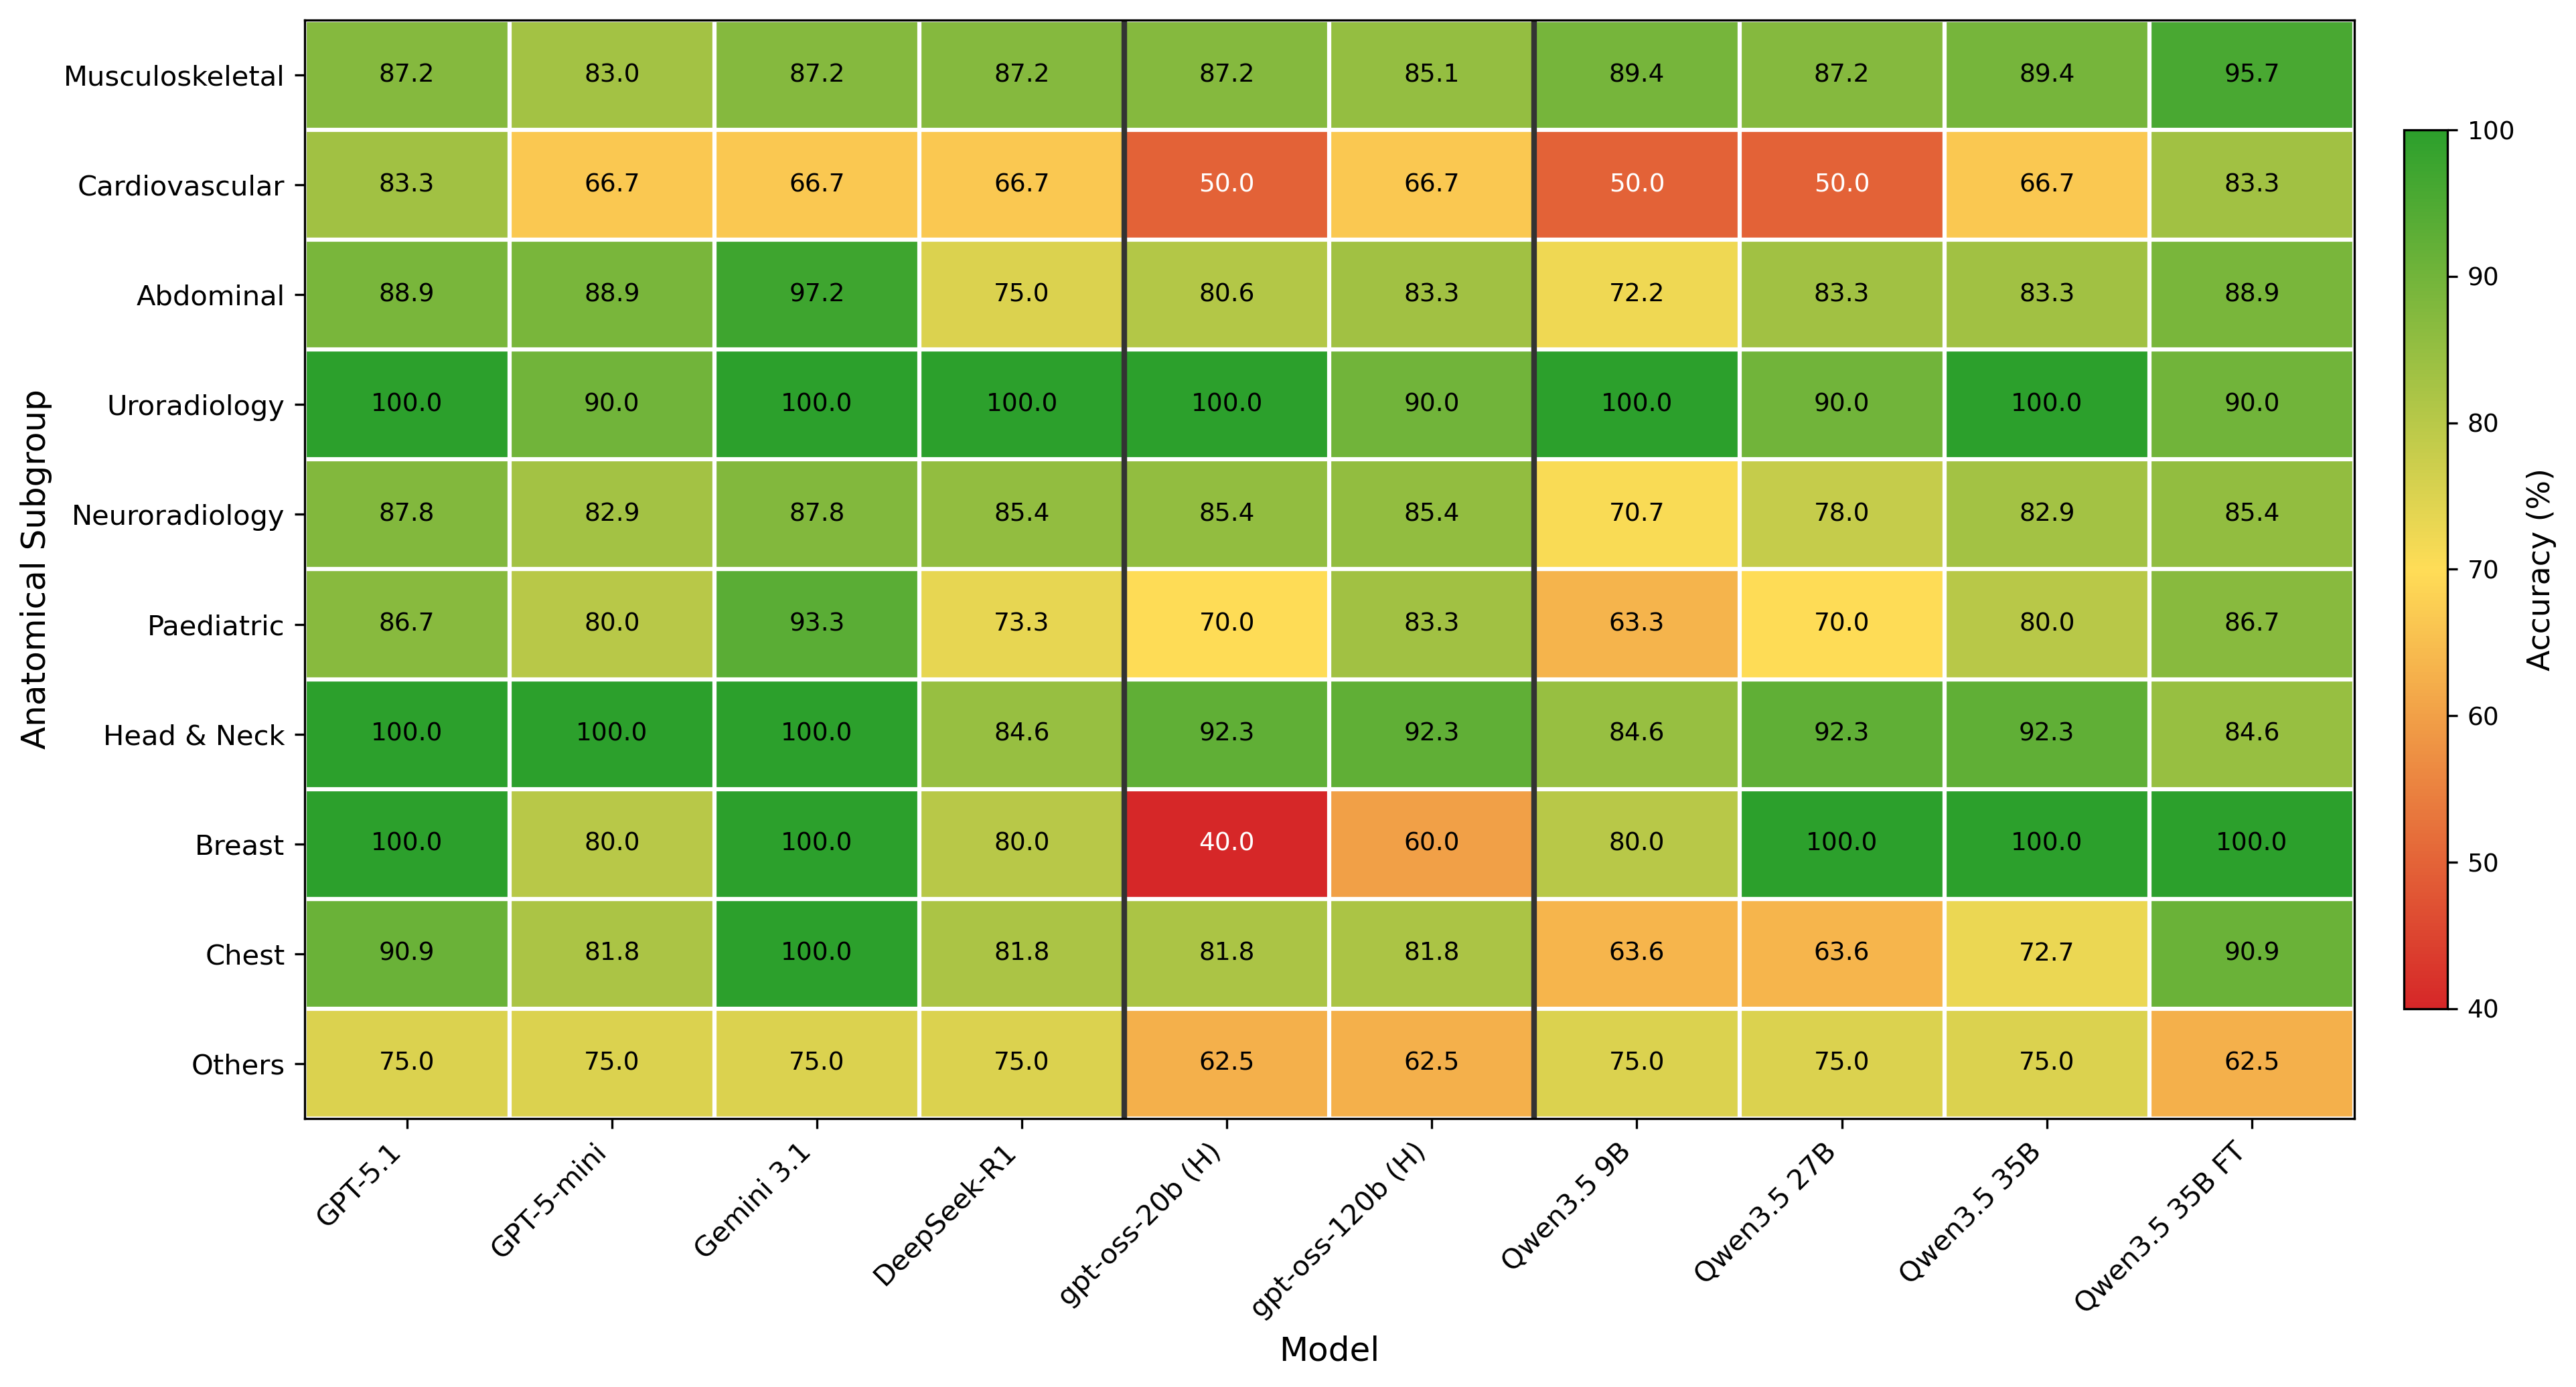
\includegraphics[width=\textwidth]{main-imgs/fig3.png}
\caption{\textbf{Heatmap of diagnostic accuracy across anatomical subgroups and model architectures.}
Color intensity represents accuracy (Green=High, Red=Low). Base on-device models from the gpt-oss, Qwen3.5, and Gemma 4 families (middle columns) exhibit variable performance across specialized domains, with degradation in areas such as Cardiovascular and Breast imaging. Fine-tuning the 20b model (far right column) effectively mitigates these domain-specific weaknesses, restoring performance levels comparable to the 120b parameter models and proprietary baselines.}
\label{fig:3}
\end{figure}

% In Primary Cardiac Lymphoma (Case 2), the base model incorrectly diagnosed angiosarcoma by overlooking third-degree AV block as a pathognomonic feature, while the fine-tuned model immediately recognized AV node encasement and systematically excluded angiosarcoma. In NICE lesions (Case 3), the base model's circular reasoning led to misdiagnosis of subacute infarcts despite absent diffusion restriction, while the fine-tuned model identified post-procedural timing as the key diagnostic clue. Across all cases, fine-tuned models demonstrate adaptive reasoning by tailoring analytical structures to diagnostic complexity. 


% The quantitative performance metrics presented in Supplementary Figures 1--4 further validate these qualitative observations of systematic reasoning. Forest plot comparisons demonstrate that the fine-tuned gpt-oss-20b model achieves 86.5\% overall accuracy, surpassing both the significantly larger DeepSeek-R1 (81.6\%, Supplementary Fig. 1) and the cloud-based o4-mini (84.1\%, Supplementary Fig. 2), while approaching the performance of the state-of-the-art GPT-5 model (88.9\%, Supplementary Fig. 3). Notably, confidence intervals overlap substantially across the majority of anatomical subgroups when compared to GPT-5, indicating statistical parity in domains such as musculoskeletal, abdominal, and neuroradiology---precisely the categories exemplified in our case studies. 


% The combination of quantitative superiority and qualitative reasoning capabilities---as demonstrated through the systematic elimination logic and adaptive analytical structures in Supplementary Cases 1--3---establishes that targeted domain adaptation can transform lightweight on-device models into clinically viable diagnostic support tools. These findings collectively demonstrate that parameter efficiency and reasoning quality are not mutually exclusive, and that appropriately fine-tuned smaller models can deliver performance comparable to substantially larger proprietary systems while maintaining the advantages of local deployment and data privacy.

The substantial performance gains across both model families demonstrate that targeted domain adaptation can effectively compensate for the smaller scale of on-device models. The fine-tuned gpt-oss-20b and Qwen3.5-35B models exhibit diagnostic accuracy comparable to significantly larger proprietary systems while retaining the advantages of local deployability and privacy preservation. These findings highlight the strong potential of lightweight, fine-tuned on-device LLMs to provide high-quality clinical decision support in settings with limited computational resources.






\section*{Methods}

\subsection*{Dataset curation and pre-processing}
Case reports for the LLM-as-a-generalist task were curated from the European Society of Radiology (Eurorad)~\cite{kottlors2025eurorad}  (\url{https://www.eurorad.org/}) database across a broad spectrum of subspecialties, including musculoskeletal, cardiovascular, abdominal, uroradiology, neuroradiology, paediatric, head and neck, breast, and chest imaging.
To strictly mitigate data leakage, the test set was restricted to cases published in 2025, postdating the training cut-off of the evaluated models. From an initial pool of 350 prospective test cases, we employed GPT-5.1 to screen and exclude reports containing explicit diagnostic disclosures in the description. Historical cases published prior to 2025 were allocated for fine-tuning, yielding a final dataset comprising 1,895 training cases and 207 independent test cases.

Cases for the LLM-as-a-specialist task were based on the recent ophthalmology multiple-choice question dataset~\cite{ophthalmologyQA}. It contains 130 questions covering six topics: anterior segment diseases, external eye/orbital diseases, glaucoma, ocular trauma, refractive disorders/strabismus, and retinal diseases. Each question has one to six correct answers from five to nine answer choices.

Cases for the LLM-as-a-clinical-judge scoring task were curated from the benchmark data in~\cite{eval-deepseek125Patients}, comprising 125 patient cases. 
Each case included a chief complaint and up to five diagnostic or treatment recommendations generated by distinct models, including GPT-4, GPT-4o, GPT-3.5, Gem2FTE, and DeepSeek-R1. In this task, the evaluated LLMs were required to audit these predictions by assigning quality scores rather than generating de novo diagnoses. Performance was assessed by measuring the concordance between model-generated scores and reference ratings provided by medical experts.

\subsection*{Task-specific inference protocols}

To ensure fair comparison, we developed standardized zero-shot inference pipelines for each clinical task. All protocols utilized a self-consistency framework where each case was queried three independent times (\(k = 3\)).

\textbf{General Radiology Diagnosis.}
The LLM-as-a-generalist diagnostic task was formulated as a constrained single-label selection problem (Supplementary Prompt 1). Models were provided with the patient history and imaging findings and instructed to select the most likely diagnosis strictly verbatim from a provided differential list. Post-processing utilized a deterministic regex-based extractor to isolate the final diagnosis from the generated reasoning stream.

\textbf{Ophthalmology Specialty QA.}
The LLM-as-a-specialist task involved complex multiple-choice questions (MCQs) requiring multi-label classification. Unlike the radiology task, models were instructed to ``Select ALL correct answers'' from options A–Z. The system prompt enforced a strict output format consisting only of concatenated capital letters (e.g., ``ABE'' or ``D''), prohibiting explanatory text in the final output to facilitate automated parsing  (Supplementary Prompt 2).

\textbf{Clinical Judgment Simulation.}
The LLM-as-a-clinical-judge task evaluated the models' ability to simulate expert clinical judgment. Models were presented with a clinical case adapted from ~\cite{eval-deepseek125Patients}, alongside a candidate diagnosis/treatment plan, and a reference standard. They were instructed to assign a quality score on a 5-point Likert scale (1 = Most relevant options missing, 5 = All relevant options mentioned) based on a strict scoring rubric. Half-point scores (e.g., 4.5) were permitted to capture granular distinctions in quality  (Supplementary Prompt 3).

\subsection*{Inference Protocol for Zero-shot Experiments}

We benchmarked three distinct categories of models to represent the current landscape of LLMs:

\textbf{Proprietary Frontier Models (GPT-5.1, GPT-5-mini, and Gemini 3.1 Pro).}
We selected OpenAI’s \texttt{gpt-5.1-2025-11-13} and \texttt{gpt-5-mini} reasoning models, alongside Google’s \texttt{gemini-3.1-pro}. These models represent the current state-of-the-art in closed-source reasoning. Inference for OpenAI models was conducted via the OpenAI Responses API, while Gemini 3.1 Pro was accessed through the Google AI API. To evaluate the impact of inference-time compute on OpenAI models, we modulated the \texttt{reasoning\_effort} parameter (\texttt{low}, \texttt{medium}, \texttt{high}). For all tasks, we utilized the default \texttt{medium} effort setting.

\textbf{Open-Source State-of-the-Art Model (DeepSeek-R1).}
To represent the pinnacle of open-source capability, we evaluated the 671-billion parameter \texttt{DeepSeek-R1-0528}. This model utilizes large-scale reinforcement learning to optimize reasoning paths and is currently the strongest non-proprietary baseline available. Inference was performed via the OpenRouter API. We utilized a context window of 8{,}192 tokens to strictly enforce the capture of the model's native reinforcement-learning-aligned reasoning traces. 

\textbf{On-Device Models (gpt-oss, Qwen3.5, and Gemma 4).}
The primary focus of this study is on-device LLMs from two model families. From the \texttt{gpt-oss} family, we evaluated both the 20-billion parameter variant (optimized for consumer GPUs) and the 120-billion parameter variant. The gpt-oss models were evaluated using the Hugging Face Inference Router, targeting the Fireworks AI provider for the 20b model and Cerebras for the 120b model to maximize throughput. Similar to the proprietary OpenAI models, we modulated the \texttt{reasoning\_effort} parameter (\texttt{low}, \texttt{medium}, \texttt{high}) through the system prompt to trigger extended chain-of-thought generation patterns. From the Qwen3.5 family, we evaluated three model sizes: 9B, 27B, and 35B parameters, as well as a fine-tuned 35B variant. The Qwen3.5 models were accessed via the Hugging Face Inference Router with high reasoning effort. Output parsing relied on a custom regex extractor to identify valid answer sequences within the generated text.
From the Gemma family, we evaluated Gemma 4 31B, Google's open-weight on-device model. Inference was performed via the Hugging Face Inference Router using the same self-consistency protocol ($k=3$). Output parsing used the same regex-based extractor applied to other on-device models.




\subsection*{Training Dataset Preparation for Radiological Cases}

The gpt-oss family consists of reasoning-capable language models designed to generate structured Chain-of-Thought (CoT) reasoning during inference. To develop high-quality training data for fine-tuning gpt-oss-20b on radiological diagnosis tasks, we employed gpt-oss-120b---a substantially larger model from the same architectural family---to curate systematic diagnostic reasoning data for all 1,895 cases in the Eurorad dataset. The use of gpt-oss-120b for data curation was predicated on three key advantages: (i) architectural consistency between the 120b and 20b variants ensures compatibility of reasoning patterns, (ii) the larger parameter count enables more sophisticated medical reasoning and systematic differential diagnosis evaluation, and (iii) automated generation provides scalable, consistent reasoning data across the entire dataset.

For each radiological case, gpt-oss-120b was provided with the clinical case presentation (comprising patient history and imaging findings), the original expert radiologist discussion from the Eurorad dataset as contextual grounding, and the list of differential diagnoses. The original discussion, which provided academic descriptions of case characteristics and imaging findings, served as reference material to inform the generation of improved systematic reasoning. The model was instructed to generate Chain-of-Thought reasoning following a structured four-step diagnostic framework: (1) symptom-finding correlation---establishing connections between clinical presentation and imaging observations, (2) differential mapping---evaluating how imaging findings support or contradict each candidate diagnosis, (3) systematic elimination---providing explicit reasoning for excluding less likely diagnostic options, and (4) diagnostic convergence---demonstrating the logical pathway to the final diagnosis. Reasoning generation employed the following parameters: temperature = 0.6, maximum output tokens = 2000, target length = 200--400 words, accessed via the HuggingFace Inference API.

Generated reasoning samples underwent systematic validation to ensure data quality. We verified that all 1,895 generated reasoning chains converged to the correct ground truth diagnosis, confirming alignment between the model's reasoning process and the clinically validated diagnoses. Automated quality metrics assessed each response for: (i) appropriate length (200--600 words acceptable range), (ii) presence of all four required reasoning components (symptom-finding correlation, differential mapping, systematic elimination, and diagnostic convergence), and (iii) response completeness (absence of premature truncation). Additionally, a subset of cases was manually inspected to validate that the systematic elimination reasoning across all four reasoning phases logically progressed toward the correct diagnosis, and that the final diagnosis selection matched the ground truth. For this subset, the generated reasoning was also compared against the original discussions to ensure clinical accuracy and logical coherence. The complete dataset comprising all 1,895 cases was used for gpt-oss-20b fine-tuning.

\subsection*{Training Protocol}
Fine-tuning of the gpt-oss-20b (M) model was performed using a curated reasoning dataset generated by its larger counterpart, gpt-oss-120b. This approach ensured that the smaller model learned from systematic diagnostic patterns that were architecturally compatible with its native reasoning framework. The model was loaded using the Unsloth framework with 4-bit quantization to enable efficient training on limited computational resources. A maximum sequence length of 4,096 tokens was configured to accommodate the clinical case presentations and associated reasoning chains.

Parameter-efficient fine-tuning was implemented using Low-Rank Adaptation (LoRA) with rank r=32 and alpha=64, targeting all linear layers in the model architecture, including query, key, value, and output projections, as well as the feed-forward network components (gate, up, and down projections) across all 32 transformer layers~\cite{hu2022lora, gao2025loraperiop,le2025impact}. Additionally, expert layers within the mixture-of-experts architecture were targeted at strategic depths: early layers (0-7) for initial processing, middle layers (8-15) for pattern recognition and reasoning, upper layers (16-23) for deep reasoning, and deep layers (24-31) for final refinement and output generation. This comprehensive targeting strategy ensured that the model could effectively learn diagnostic reasoning patterns at multiple levels of abstraction. A LoRA dropout rate of 0.05 was applied to prevent overfitting, and gradient checkpointing was enabled to reduce memory consumption during training.

The curated reasoning data was formatted using the gpt-oss chat template with medium reasoning effort, incorporating the gpt-oss-120b-generated reasoning as structured thinking content. This approach enabled the model to learn from the systematic diagnostic patterns demonstrated by the larger model while maintaining compatibility with the gpt-oss reasoning framework. Training was conducted over 3 epochs using the AdamW optimizer with a learning rate of $1 \times 10^{-4}$, cosine learning rate scheduling, and a warmup ratio of 0.1. 

In parallel, fine-tuning of the Qwen3.5-35B-A3B model was conducted to evaluate the adaptability of the Qwen family. Because different model families exhibit distinct intrinsic reasoning styles, we curated a separate reasoning dataset generated specifically by the larger Qwen3.5-122B model to maintain alignment and prevent formatting clashes during training. To ensure optimal training stability, the Qwen3.5 model was loaded in 16-bit precision (bfloat16) without 4-bit quantization, in accordance with Unsloth documentation advising against MoE QLoRA for this specific architecture. The maximum sequence length was adjusted to 2,048 tokens to safely manage memory scaling constraints. LoRA was applied globally to key attention and feed-forward modules with a rank of r=16 and alpha=32. A LoRA dropout rate of 0 was strictly enforced to maintain compatibility with the MoE expert layer parameter wrappers, alongside Unsloth-optimized gradient checkpointing. The data was formatted using the Qwen3.5 chat template, with structured diagnostic reasoning steps embedded explicitly within <think> tags. Training utilized the 8-bit AdamW optimizer over 3 epochs with a reduced learning rate of 5e-5, maintaining the cosine scheduling and 0.1 warmup ratio.

For both models, mixed-precision training with bfloat16 was utilized to accelerate computation while maintaining numerical stability, and all experiments were conducted with fixed random seeds to ensure reproducibility.


\subsection*{Inference protocol of fine-tuned models}

To evaluate the fine-tuned models on radiological diagnosis, we employed tailored inference strategies to account for the differing baseline capacities of the underlying architectures. For the smaller gpt-oss-20b model, we designed a controlled inference pipeline optimized for the exploration of deterministic and diverse hypotheses. Our goal was to demonstrate that advanced inference strategies can be leveraged to further boost the performance and reliability of highly constrained models. All predictions for this model were generated using group beam search, a decoding strategy that encourages exploration across diverse reasoning paths while maintaining stability in high-stakes clinical settings. After systematic experimentation with different decoding settings, we found that a configuration of 13 beams, 13 beam groups, and a diversity penalty of 0.5 provided the strongest performance on the Eurorad validation set. This setup enforced full beam-group separation, ensuring that each beam starts its own reasoning trajectory and looks at the presented case from a different angle, which is particularly effective in reducing mode collapse and repetitive reasoning. Maximum generation length was set to 3,000 tokens to accommodate longer Chain-of-Thought outputs, and sampling was disabled to ensure reproducibility across runs.

For each case, the gpt-oss-20b model produced 13 independent reasoning traces. Final predictions were obtained using a majority-vote aggregation over the extracted diagnostic answers, with ties resolved by selecting the earliest beam. All inputs were encoded with the gpt-oss chat template using left padding and a 4,096-token context window, and inference was executed using the Unsloth runtime with 4-bit quantized weights and attached LoRA adapters. This protocol allowed the model to balance the range of diagnostic reasoning with reliability, resulting in a stable exact-match performance while preserving a clinically interpretable diagnostic rationale.

Conversely, the fine-tuned Qwen3.5-35B model demonstrated robust diagnostic reasoning without the need for additional decoding strategies. Inference was conducted using the Unsloth runtime with 4-bit quantization. Inputs were processed within a 2,048-token maximum sequence length. We employed standard autoregressive generation with a temperature of 0.7 and a maximum generation length of 4,000 tokens to safely accommodate its extensive, multi-phase chain-of-thought outputs. This contrast in inference protocols highlights that while advanced search strategies are valuable for extracting maximal performance from smaller models, other models can achieve state-of-the-art clinical accuracy using default inference configurations.




\subsection*{Statistical analysis}
To account for the stochastic nature of Large Language Model (LLM) generation, we employed a self-consistency framework wherein each model was queried three independent times ($k=3$) for every case. All performance metrics and statistical comparisons were derived from the consensus prediction of these three runs. For nominal tasks, including the general diagnosis questions and ophthalmology specialty-specific questions, the consensus was determined via majority voting, where a prediction was considered correct only if the correct answer was generated in at least two of the three runs. For ordinal tasks evaluated on a 5-point Likert scale (LLM-as-a-judge for diagnosis and treatment scoring), the consensus was defined as the mean score of the three runs to obtain a stable per-case consensus score.

Model performance for nominal tasks was reported as accuracy, with 95\% Confidence Intervals (CIs) calculated using the Wilson Score Interval method to provide robust estimates for binomial proportions. For the clinical judge task, performance was reported as the signed median error across cases between the model’s mean consensus score and the ground-truth human expert score, summarized using the interquartile range (IQR). Statistical significance between model performances was determined using pairwise hypothesis tests on paired samples evaluated on the same test cases, with a significance threshold of $P < 0.05$. Differences in accuracy for nominal tasks were assessed using McNemar’s Test with continuity correction, while differences in the distribution of errors for ordinal clinical judgment tasks were assessed using the Wilcoxon Signed-Rank Test.

We further evaluated both the internal stability of the models and agreement between models using metrics appropriate to the nominal and ordinal structure of the evaluation tasks. To measure generation consistency across the three inference runs (intra-model stability), we calculated Fleiss’ Kappa ($\kappa$) for nominal datasets and the Intraclass Correlation Coefficient (ICC, form 3,k) for ordinal datasets. To assess the degree to which different models converged on identical predictions independent of ground truth (inter-model agreement), we calculated standard Cohen’s Kappa for nominal tasks. For ordinal LLM-as-a-judge scoring tasks, Linear Weighted Kappa was employed to penalize partial disagreements (e.g., scores of 4 vs. 5) less severely than complete disagreements.


\section*{Discussion}

This study systematically evaluates the capabilities of on-device large language models across three representative clinical tasks: general diagnosis, specialty-level reasoning, and simulation of expert judgment. Across all settings, the gpt-oss, Qwen3.5, and Gemma 4 models demonstrate clinically meaningful performance despite their substantially smaller scale relative to frontier proprietary models (such as GPT-5.1, GPT-5-mini, and Gemini 3.1 Pro), underscoring the feasibility of deploying lightweight LLMs directly within healthcare institutions.

In the general disease diagnosis task, on-device models achieved strong zero-shot performance, showing that compact architectures can capture the broad clinical reasoning patterns required for diagnosis. Notably, the Qwen3.5-35B base model matched the proprietary GPT-5-mini (84.5\% vs 84.1\%), while the 27B variant (80.2\%) performed comparably to DeepSeek-R1 (81.6\%), demonstrating that multiple on-device architectures can independently achieve strong clinical reasoning. Gemma 4 31B further extended this pattern, achieving the strongest base on-device accuracy (86.5\%) without fine-tuning and exceeding GPT-5-mini. The consistency of strong performance across three independent model families suggests that the viability of locally deployable clinical decision support is not contingent on a specific architecture. Moreover, in the ophthalmology specialty task, the on-device gpt-oss-120b model outperformed both GPT-5.1 and GPT-5-mini while ranking third overall behind Gemini 3.1 Pro and DeepSeek-R1. This is noteworthy given that most existing clinical LLM evaluations have focused on large cloud-based models~\cite{zhang2025ophthreview, bhayana2024radiology, schramm2025multimodal}, leaving open the question of whether smaller locally deployable systems can achieve comparable levels of generalization. Our findings indicate that modern on-device architectures can support robust performance in common diagnostic scenarios without requiring external computation or data transfer.

The ability of LLMs to act as "clinical judges" is critical for scalable quality assurance and automated evaluation~\cite{kocaman2025clever, croxford2025evaluating}. Our results indicate that on-device models can align closely with human expert consensus, often exhibiting greater stability than efficient proprietary alternatives like GPT-5-mini. All three Qwen3.5 models achieved median diagnostic errors of 0.00, matching the best-performing models and confirming that lightweight architectures can reliably simulate expert judgment. This suggests that compact models can support evaluative tasks that require not only factual knowledge but also sensitivity to clinical reasoning standards and rubric-based assessment criteria. This capability is essential for deploying LLMs as automated auditors or second-opinion systems in clinical workflows~\cite{humaneval2025llmjudge, genovese2026artificial}.

Beyond zero-shot performance, the adaptability of on-device models represents a substantial advantage over closed-source systems. Fine-tuning the gpt-oss-20b and Qwen3.5-35B models on general diagnosis data substantially improved their performance, with the fine-tuned Qwen3.5-35B achieving an exact match accuracy of 88.4\% (95\% CI: 83.3--92.1\%), closely rivaling GPT-5.1 (88.9\%). We observed that fine-tuning yielded the most robust improvements when models were trained on reasoning traces generated by a larger, architecturally matched model from the same family (e.g., utilizing Qwen-122B for the Qwen3.5 series, and gpt-oss-120b for the gpt-oss series). Because different model families exhibit intrinsic variations in how they structure logic, this family-matched approach preserves the native reasoning style, preventing formatting clashes and optimizing the assimilation of systematic diagnostic patterns. This result suggests that domain-specific optimization, when aligned with a model's inherent reasoning architecture, can efficiently compensate for smaller model scale~\cite{davis2026medslice, guluzade2025elmtex, wind2025rar}. Fine-tuning also enhanced robustness across radiology subspecialties, yielding more uniform performance and mitigating weaknesses observed in the base models. These findings highlight that clinics can deploy efficient, low-cost, customized AI tools tailored to their specific patient demographics and disease prevalences without compromising data privacy.

Taken together, the experiments in this study highlight three key insights. First, compact on-device LLMs across multiple model families (gpt-oss, Qwen3.5, Gemma 4) can provide strong general diagnostic reasoning and domain-specific performance. Second, on-device LLMs can approximate expert judgment with surprising fidelity, positioning them as valuable components of locally governed AI ecosystems that support both clinical decision-making and meta-evaluative tasks. Third, fine-tuning plays a critical role in achieving competitive accuracy across diverse subspecialties, allowing healthcare institutions to develop tailored high-performing models from relatively small architectures.

Our study also has limitations. First, while our benchmarks cover diagnosis, management, and evaluation, they rely on retrospective patient cases and examination questions, which may not fully capture the complexity and noise of real-time clinical environments. Local deployment mitigates privacy and data governance concerns but introduces operational challenges, including hardware reliability, secure integration with clinical information systems, and ongoing monitoring of model behavior~\cite{asgari2025hallucination, omar2025adversarial}. Fine-tuning requires access to high-quality labeled data, which may be limited in certain specialties. Building on our findings regarding model-specific logic patterns, part of our future work will explore the variations in intrinsic reasoning styles between different vendors. Specifically, investigating multi-vendor, agentic debate frameworks—where diverse models collaborate, critique, or iteratively refine each other's diagnostic reasoning—could provide a novel mechanism to further enhance accuracy and reliability in highly complex clinical scenarios.

In summary, this work demonstrates that on-device LLMs offer a promising and practical alternative to large proprietary systems for clinical decision support. These compact models can achieve reliable diagnostic reasoning, robust subspecialty performance, and alignment with expert judgment---all while maintaining strict control over patient data and computational infrastructure. These features position on-device LLMs as strong candidates for safe, scalable, and equitable integration of AI into clinical practice.


\subsection*{Data Availability}
The benchmarking results and model outputs generated in this study are available in the Supplementary Information. The raw input data for the general diagnosis task are available from the Eurorad library (\url{https://www.eurorad.org/}); a script to retrieve the specific cases used in this study is provided in the code repository. The ophthalmology and clinical judge datasets are publicly available at \url{https://github.com/bowang-lab/on-device-LLM}. The training dataset with gpt-oss-120b reasoning enhancement used to fine-tune the model is available at \url{https://huggingface.co/datasets/wanglab/eurorad-gpt-oss-training-data}.

\subsection*{Code Availability}
The code for model inference, benchmarking, and evaluation is publicly available on GitHub at \url{https://github.com/bowang-lab/on-device-LLM}. The fine-tuned model weights are available on HuggingFace at \url{https://huggingface.co/wanglab/on-device-LLM-gpt-oss-20b}.

\subsection*{Acknowledgements} 
This work was supported by the Natural Sciences and Engineering Research Council of Canada (RGPIN-2020-06189 and DGECR-2020-00294) and CIFAR AI Chair programs. This research was enabled, in part, by computing resources provided by the Digital Research Alliance of Canada. 


% \subsection*{Supplementary}















\bibliographystyle{IEEEtran}
\bibliography{main-ref}

\end{document}


